This chapter sets the rules used to turn simulator output into thesis evidence. The datasets and their permitted claims are defined first (Section~\ref{sec:analysis_datasets}), followed by the architecture and scenario design (Sections~\ref{sec:architecture_design}--\ref{sec:scenario_design}), integrity and eligibility tests (Sections~\ref{sec:integrity_gate}--\ref{sec:analysis_populations}), and the statistical and decision analysis (Section~\ref{sec:statistical_workflow}). Chapters~6 and~7 follow this order. Commands and repository operation are left to Appendix~E because they are needed for reproduction but are not part of the scientific argument.

\section{Analysis Datasets and Permitted Inference}
\label{sec:analysis_datasets}

The report uses one final Fresh V2 campaign together with the earlier Reference Campaign. Within Fresh V2, comparison blocks are selected according to the claim being tested rather than pooled without regard to task population or fleet coverage.

\begin{table}[htbp]
\centering
\caption{Analysis datasets and the claims they can support.}
\label{tab:evidence_layers}
\begin{tabularx}{\textwidth}{L{0.22\textwidth}L{0.27\textwidth}Y}
\toprule
Dataset & Coverage & Permitted use \\
\midrule
Reference Campaign & 891 California and 891 India architecture cases & Historical matched event-window baseline under the frozen nominal model \\
Fresh V2 regional block & 594 California and 594 India cases at 60/120 satellites; 539 scenarios per case & Paired event-window effects, failure sensitivity, exact Pareto analysis, and cross-window candidates \\
Fresh V2 India 180-satellite extension & 282 verified cases on 773 tasks; balanced 216-case CN30--CN100 block & Large-fleet response, matched India 120-to-180 effects, robustness, priority timing, and portfolio extension \\
\bottomrule
\end{tabularx}
\end{table}

The Reference Campaign predates the Fresh V2 scenario contract. It is retained because it provides a complete like-for-like sweep under one frozen model, but its values are not averaged with Fresh V2. The final Fresh V2 campaign contains a matched regional block and an India 180-satellite extension. California and India share 594 architecture identifiers in the 60/120-satellite block, while the 180-satellite cases use the same 773-task India contract. The complete CN30--CN100 part can therefore be paired with the corresponding 120-satellite architectures for a fleet-size contrast. California--India conclusions remain limited to 60/120 satellites because no California 180-satellite population was executed.

\section{Architecture Design}
\label{sec:architecture_design}

Four geometry factors produce 81 base architectures. Each base geometry is evaluated at eleven Central Node fractions, giving 891 identifiers per event window. Table~\ref{tab:factor_grid} lists the factors and explains what their variation represents.

\begin{table}[htbp]
\centering
\caption{Architecture factors in the Full891 design.}
\label{tab:factor_grid}
\begin{tabularx}{\textwidth}{L{0.25\textwidth}L{0.28\textwidth}Y}
\toprule
Factor & Levels & Experimental role \\
\midrule
Total satellites & 60, 120, 180 & Fleet scale and resource proxy \\
Orbital planes & 3, 5, 10 & Spatial distribution and temporal contact geometry \\
Altitude & 500, 800, 1000 km & Access and communication opportunity \\
Inclination & 60, 80, 98.6 deg & Latitude-dependent access geometry \\
Central Node fraction & 0, 10, $\ldots$, 100\% & Exposure to the implemented Central Node routing package \\
Walker phasing & $F=1$ & Fixed control \\
\bottomrule
\end{tabularx}
\end{table}

The factorial grid makes matched contrasts possible: a Central Node fraction can change while the Walker geometry remains fixed, and a California result can be paired with the same case identifier in India. The Central Node treatment is nevertheless a package. It changes eligibility, forwarding preference, deterministic placement, and link-budget assumptions together. Consequently, a response to Central Node fraction is a response to that implemented package, not an isolated causal coefficient for a single mechanism.

\section{Scenario Design}
\label{sec:scenario_design}

Fresh V2 declares 539 scenario identifiers for every architecture (Table~\ref{tab:v2_scenario_matrix}). Deterministic settings are evaluated once. Random failure families use 30 seeded trials at each severity; combined-stress cells use 10. A replicate changes only the seeded failed nodes, removed windows, or outage interval while retaining architecture, task set, family, and severity.

\begin{table}[htbp]
\centering
\small
\caption{Fresh V2 scenario contract for each architecture case.}
\label{tab:v2_scenario_matrix}
\begin{tabularx}{\textwidth}{L{0.30\textwidth}L{0.45\textwidth}r}
\toprule
Scenario family & Construction & Rows \\
\midrule
Core, policy, and unlimited & Seven named scenarios & 7 \\
Task size & $0.5\times$, $1\times$, $2\times$, $4\times$ & 4 \\
Random satellite failure & Four levels $\times$ 30 trials & 120 \\
Random Central Node failure & Four levels $\times$ 30 trials & 120 \\
Link-window outage & Four levels $\times$ 30 trials & 120 \\
Ground-station outage & Four levels $\times$ 30 trials & 120 \\
Targeted Central Node failure & Four deterministic levels & 4 \\
Capacity degradation & Four deterministic levels & 4 \\
Combined stress & Two packet sizes $\times$ two failure levels $\times$ 10 trials & 40 \\
\midrule
Total & & 539 \\
\bottomrule
\end{tabularx}
\end{table}

Thirty trials per random-failure level are used for mean-response comparisons. The combined-stress cells have only ten trials, so they are used descriptively without a reported fifth-percentile or fine rank order. A convergence extension would be needed for that purpose. Central Node failure at CN0 is stored as \texttt{NOT\_APPLICABLE}. Keeping this row prevents an experiment that has no meaning at CN0 from being confused with a failed simulation.

\section{Scientific Analysis Workflow}
\label{sec:analysis_workflow}

Figure~\ref{fig:analysis_workflow} gives the order applied to every result. Input identity and integrity are checked before a plot, score, or ranking is calculated. If a gate fails, the population is either restricted to a valid comparison block or the claim is withheld. Normalization and weighting are not used to conceal an incomplete input or output.

\begin{figure}[htbp]
\centering
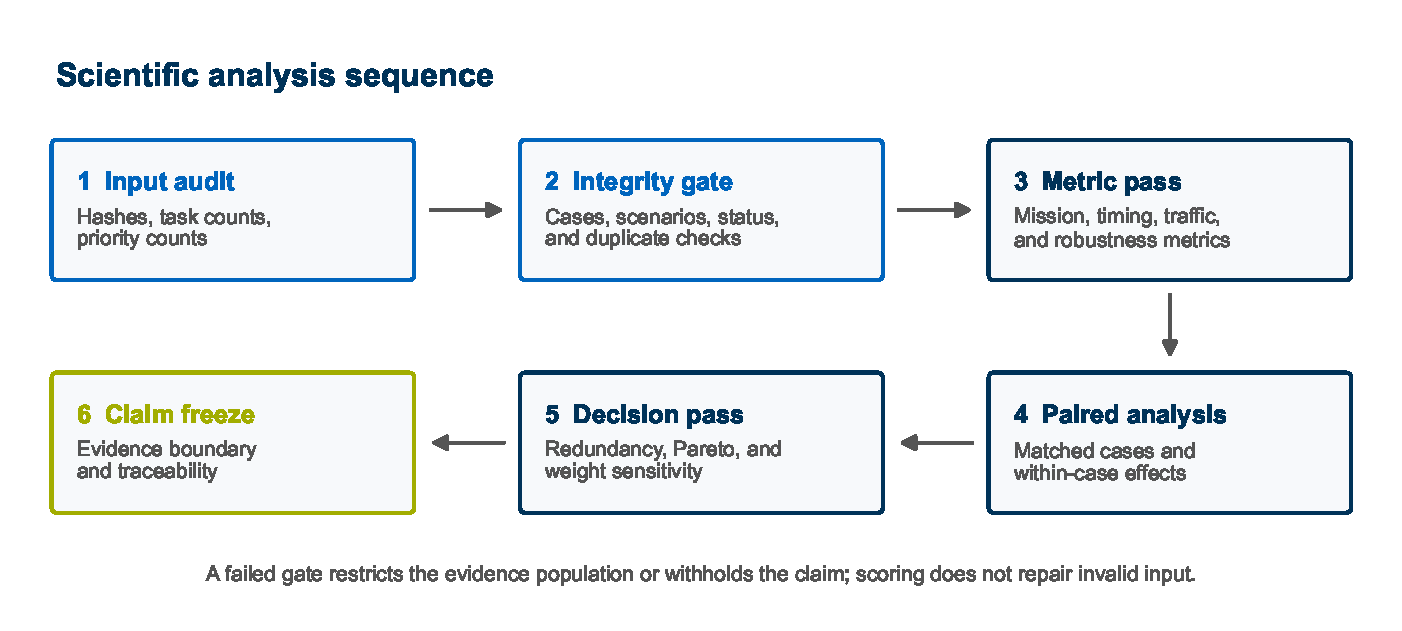
\includegraphics[width=\textwidth]{part2_revision/01_analysis_workflow.pdf}
\caption{Logical sequence from input audit to a frozen thesis claim. Implementation details are documented separately in Appendix~E.}
\label{fig:analysis_workflow}
\end{figure}

Only an eligible population proceeds to the statistical and decision stages. This prevents a plausible-looking plot from hiding duplicate rows, changed denominators, an incomplete fraction sweep, or mishandled censoring. Any one of these issues can change the Pareto set and the reported architecture order.

\section{Integrity Gate and Task Provenance}
\label{sec:integrity_gate}

Fresh V2 was inventoried before any mean or contrast was calculated. A complete regional inventory should contain $891\times539=480{,}249$ case--scenario status keys, and both regional archives meet that count after validation. Restarting the California campaign had created 4,269 duplicate intermediate keys. The de-duplication rule retains the final scientifically identical record, and no retained row has a failed status. This gate follows the model-credibility principle that an input, assumption, verification result, and intended claim must be traceable; a single global ``validated'' label is not enough \citep{NASA2016SEHandbook,NASAStd7009}. Table~\ref{tab:validation_gate} lists the actual checks and their evidence.

\begin{table}[htbp]
\centering
\small
\caption{Validation gates applied before result calculation.}
\label{tab:validation_gate}
\begin{tabularx}{\textwidth}{L{0.24\textwidth}Y L{0.21\textwidth}}
\toprule
Gate & Test & Evidence \\
\midrule
Inventory & Expected case directories, 539 scenario identifiers per case, markers, and explicit not-applicable states & Appendix~C; completion-gate table \\
Uniqueness and status & Unique case--scenario keys after deterministic de-duplication; no failed retained row & Appendix~C; integrity summary \\
Input contract & SHA-256 digest, regional task counts, priority counts, and metric denominators & Appendix~C; task-population contract \\
Metric reconstruction & Independent recomputation from retained task/transfer evidence where available & Appendix~C; metric audit \\
Pair eligibility & Shared case identifiers, complete factor sweep, and identical task population for each comparison & Tables in Chapters~6--7 \\
Decision eligibility & Missing values removed explicitly; redundancy checked; exact Pareto set computed before weighting & Decision tables and manifest \\
\bottomrule
\end{tabularx}
\end{table}

The intended task file has the full SHA-256 digest
\begin{center}
\small\texttt{e717a1dde84db0f47efdda09cfca2f437}\linebreak
\texttt{909349b25a139a45a7c1928da80e533}.
\end{center}
The hashed file contains 32 California tasks and 773 India tasks. In the first India 180-satellite execution, regional filtering preserved source labels 32--804, while normalization created an index from 0--772. Label-based assignment then produced 32 invalid coordinate rows and omitted the final 32 source rows. The corrected package resets the positional index before normalization and checks both the regional count and task hashes in its run contract. Its verifier reports 282 complete cases, no missing or invalid cases, 539 scenarios per case, and all 773 India tasks. None of the earlier 741-task values is used in the final tables or figures.

\section{Analysis Populations}
\label{sec:analysis_populations}

Table~\ref{tab:analysis_population_summary} gives the final populations. The balanced blocks are used whenever marginal curves, paired effects, Pareto filtering, or rank comparisons require equal architecture coverage.

\begin{table}[htbp]
\centering
\small
\caption{Final analysis populations after the integrity gate.}
\label{tab:analysis_population_summary}
\begin{tabularx}{\textwidth}{Yrrrr}
\toprule
Population & Bases & Cases & Scenarios/case & Rows \\
\midrule
Matched California 60/120 & 54 & 594 & 539 & 320,166 \\
Matched India 60/120 & 54 & 594 & 539 & 320,166 \\
India 180, all completed & 27 & 282 & 539 & 151,998 \\
India 180, balanced CN30--CN100 & 27 & 216 & 539 & 116,424 \\
\bottomrule
\end{tabularx}
\end{table}

The 180-satellite selection contains 20 cases at CN0, 22 at CN10, 24 at CN20, and all 27 base architectures at every level from CN30 through CN100. Low-CN rows remain available for inventory and individual-case inspection, but they are excluded from aggregate rankings that require equal base weights.

\section{Metrics Used in the Main Analysis}
\label{sec:main_metrics}

The principal measures are defined here because their denominators determine the scientific interpretation. Appendix~A provides complete formulas and edge-case handling.

\begin{table}[htbp]
\centering
\small
\caption{Principal result metrics and interpretation.}
\label{tab:principal_metrics}
\begin{tabularx}{\textwidth}{L{0.24\textwidth}Y L{0.27\textwidth}}
\toprule
Metric & Meaning & Important boundary \\
\midrule
Observation fulfilment & Percentage of released tasks observed after the observing satellite received the task & Not a sensor-quality or end-to-end response metric \\
Strict useful completion (\Suseful) & Percentage of tasks delivered before deadline to every simulator-defined useful recipient & Becomes harder as the useful-recipient set grows \\
Useful-recipient coverage & Mean fraction of useful recipients reached before deadline & Complements the strict all-recipient condition \\
P100 $T_{100}$ & Worst complete-dissemination time among tasks for which every useful recipient is reached & Undefined when any required delivery misses the deadline \\
Transferred data & Total modeled task-message traffic per case & Task-message burden, not image-data volume \\
Robustness retention & Stressed metric divided by the matched unlimited baseline & A relative sensitivity measure, not failure probability \\
\bottomrule
\end{tabularx}
\end{table}

Timing analyses retain missed events as right-censored observations. Priority classes use their fixed deadline horizons, and any cross-window summary gives High, Medium, and Low equal weight rather than allowing the more numerous Low-priority tasks to dominate. The event-time summaries use the Kaplan--Meier estimator \citep{KaplanMeier1958} and restricted mean event-free time within the declared deadline horizon \citep{RoystonParmar2013}.

\section{Statistical and Decision Workflow}
\label{sec:statistical_workflow}

After the population and metric definitions are fixed, the following steps are applied in order:

\begin{enumerate}
\item \textbf{Describe the response.} Marginal means show the response over the enumerated grid. Base-clustered percentile-bootstrap intervals \citep{Efron1979} show how stable that mean is across the tested base architectures; they are not geographic-population intervals.
\item \textbf{Form matched contrasts.} Results are subtracted only within the same architecture identifier when comparing event windows or scenarios. This removes between-architecture differences from the contrast.
\item \textbf{Check association and shape.} Spearman $\rho$ measures monotonic rank agreement without requiring a straight-line relation. A regression through the eleven Central Node marginal means is used as a compact description of shape. Cross-validated error is reported so that a high in-sample $R^2$ is not mistaken for a physical law.
\item \textbf{Measure robustness.} Each disturbed case is paired with the same architecture's unlimited baseline. Raw stressed performance, change, retention, and the response over severity are shown before ranking. This keeps degradation and robustness-envelope behaviour visible instead of collapsing them into one network score \citep{Trajanovski2013,Xu2023}.
\item \textbf{Screen redundancy.} Highly correlated metrics remain in the diagnostic tables, but a near-duplicate pair does not receive two full contributions to utility.
\item \textbf{Apply exact Pareto filtering.} A case is removed if another eligible case is at least as good in every declared objective and better in one. Raw objective directions are used before any preference weights, as in Pareto-robust space-system trade studies \citep{Ridolfi2013}.
\item \textbf{Test preference sensitivity.} Dirichlet weight draws record how often a remaining case ranks first or in the top five. This is a stochastic multi-criteria acceptability analysis of the chosen preference range \citep{LahdelmaSalminen2001}; it is not a survey of stakeholder opinion. The broader principle is that a simulation conclusion should be checked against declared factor and preference changes \citep{Kleijnen2005}.
\end{enumerate}

The workflow produces a portfolio rather than a universal winner. Weighted utility is used only inside the feasible Pareto set and never substitutes for raw mission, timing, traffic, and fleet values.

\section{Scope Limits}

The evidence uses a fixed \SI{700}{\kilo\metre} access radius, one deterministic balanced Central Node placement, one ground station, one set of task-generation rules, and a bundled Central Node routing treatment. The two event windows are selected cases rather than random samples. Within the final campaign, the 180-satellite extension supports a controlled India 120-to-180 comparison only on the balanced CN30--CN100 cells and under the shared scenario definition. It does not create a California--India comparison at 180 satellites, and the incomplete CN0--CN20 selection prevents a fully balanced three-fleet sweep over all eleven fractions. These boundaries determine the wording of Chapters~7--9.
